\documentclass[12pt,xcolor=pdftex,dvipsnames,table]{beamer}
\usetheme{default}
\title{Remote Signing Service}
\author{Gabor Tanz, Patrick Hirt}
\usepackage[ngerman]{babel}
\usepackage{babelbib}
\usepackage[utf8]{inputenc}
\usepackage{graphicx}
\usepackage[T1]{fontenc}
\usepackage{cclicenses}
\usepackage{lmodern}
\usepackage{float}
\usepackage{colortbl}
\usepackage{longtable}
\usepackage{adjustbox}
\usepackage{listings}

\usepackage{tikz}
\usetikzlibrary{shapes.geometric, arrows, arrows.meta}
\tikzstyle{startstop} = [rectangle, rounded corners, minimum width=3cm, minimum height=1cm,text centered, draw=black, fill=red!30]
\tikzstyle{io} = [trapezium, trapezium left angle=70, trapezium right angle=110, minimum width=3cm, minimum height=1cm, text centered, draw=black, fill=blue!30]
\tikzstyle{process} = [rectangle, minimum width=3cm, minimum height=1cm, text centered, draw=black, fill=orange!30]
\tikzstyle{decision} = [diamond, minimum width=3cm, minimum height=1cm, text centered, draw=black, fill=green!30]
\tikzstyle{arrow} = [thick,->,>=stealth]



\newcommand{\Subitem}[1]{
{\setlength\itemindent{15pt} \item[-] #1}
}

\begin{document}

    \begin{frame}
        \titlepage
    \end{frame}

    \begin{frame}
        \frametitle{Inhalt}
        \begin{enumerate}
            \item Problemstellung
            \item Auftrag
            \item Lösungsansatz
            \item Stand
        \end{enumerate}
    \end{frame}

    \begin{frame}
        \frametitle{Problemstellung}
        \begin{columns}[T]
            \begin{column}{0.5\textwidth}
                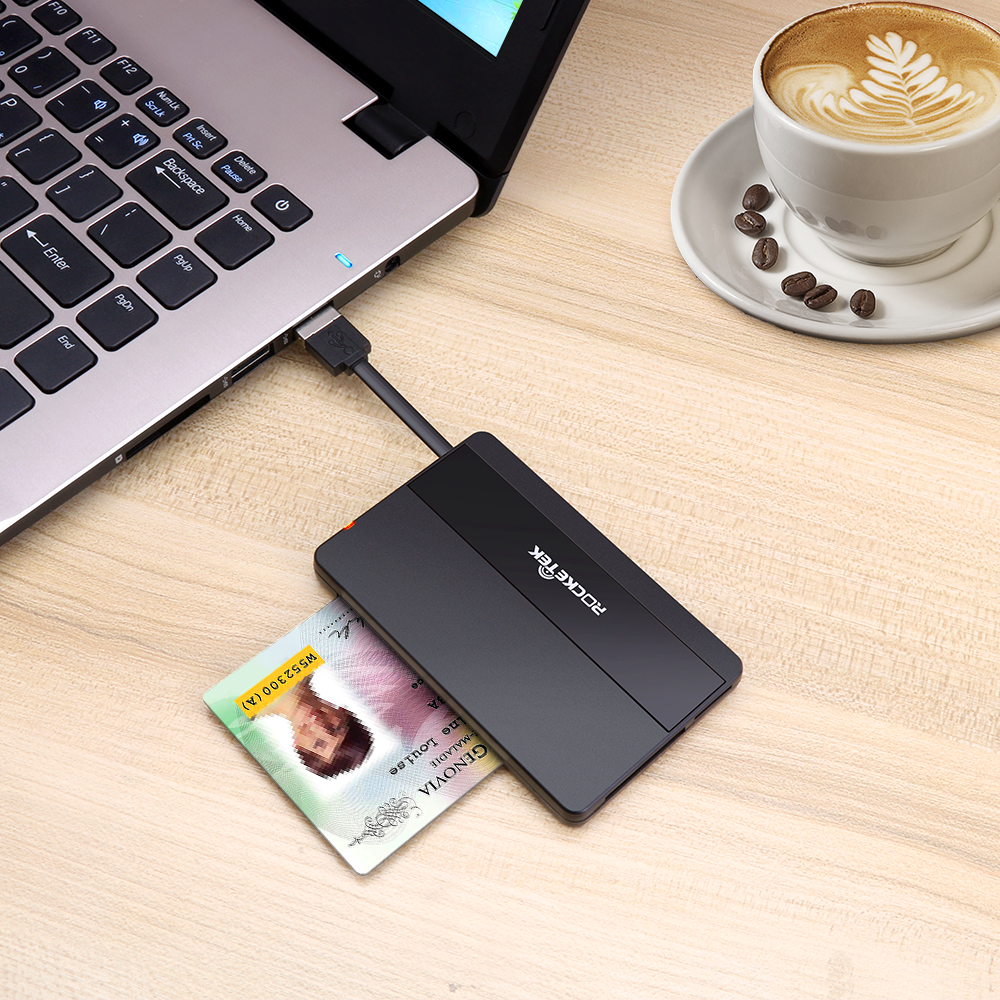
\includegraphics[width=\textwidth]{images/cardreader.jpg}
            \end{column}
            \begin{column}{0.5\textwidth}
                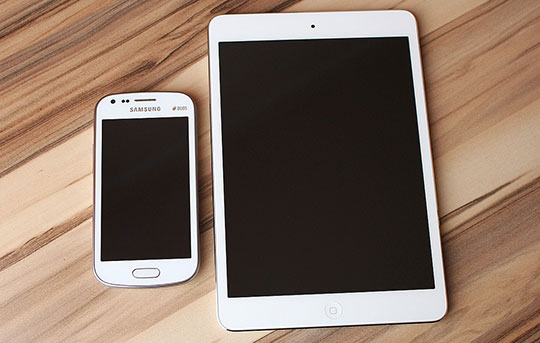
\includegraphics[width=\textwidth]{images/tablet-smartphone.jpg}
            \end{column}
        \end{columns}
    \end{frame}

    \begin{frame}
        \frametitle{Auftrag}
        \begin{itemize}
            \item Spezifikation, Konzeption und Aufbau eines Remote Signing Services basierend auf OIDC
            \item Aufbauend auf unserer Arbeit im Projekt 2
        \end{itemize}
    \end{frame}

    \begin{frame}
        \frametitle{Technologien}
        \begin{columns}[T]
            \begin{column}{0.5\textwidth}
                \begin{itemize}
                    \item Protobuf
                    \Subitem{Serialisierungsformat}
                    \Subitem{einfaches Schema}
                    \Subitem{extrem kompakt}
                    \Subitem{sehr schnell}
                \end{itemize}
            \end{column}
            \begin{column}{0.5\textwidth}
                \begin{itemize}
                    \item OIDC
                    \Subitem{Basierend auf OAuth 2}
                    \Subitem{ID Token als JWT}
                    \Subitem{Flows für verschiedene Anwendungszwecke}
                \end{itemize}
            \end{column}
        \end{columns}
    \end{frame}

    \begin{frame}
        \frametitle{Grobkonzept}
        \begin{itemize}
            \item Separate Signaturdatei, um formatsunabhängig signieren zu können
            \item Hash-Wert mit Identität verknüpfen
            \item Timestamps und Gültigkeit
            \item Signing Service generiert Zertifikate im Namen des Users
        \end{itemize}
    \end{frame}


    \begin{frame}
        \frametitle{Prozess für qualifizierte Signaturen (1/2)}

        \begin{figure}[H]
            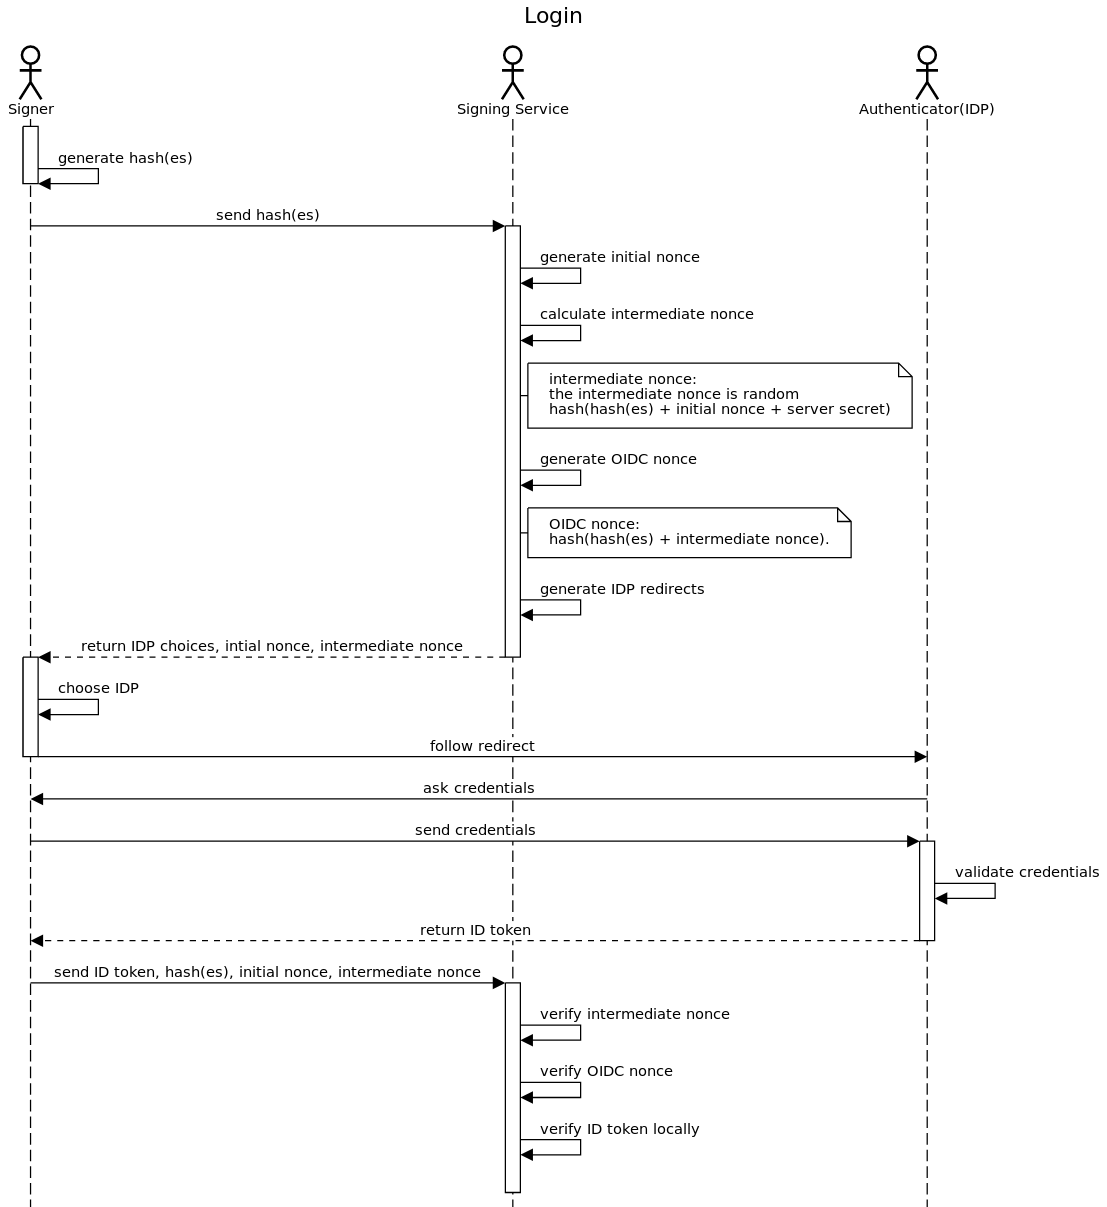
\includegraphics[scale=0.2]{images/signature_generation_step1.png}
        \end{figure}
    \end{frame}

    \begin{frame}
        \frametitle{Prozess für qualifizierte Signaturen (2/2)}

        \begin{figure}[H]
            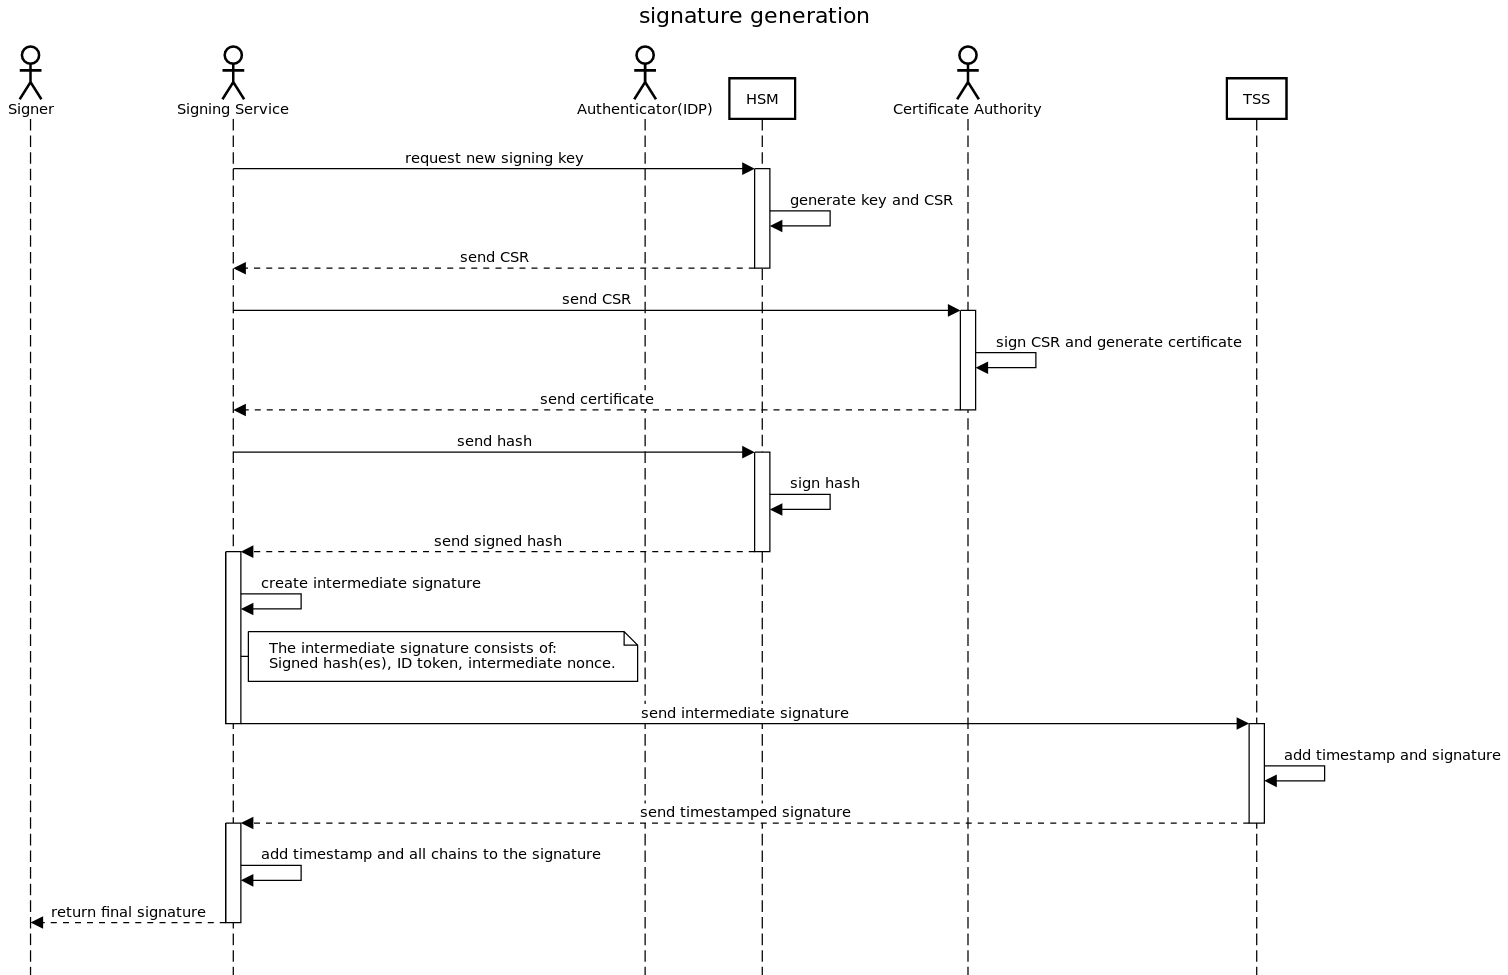
\includegraphics[scale=0.22]{images/signature_generation_step2.png}
        \end{figure}
    \end{frame}

    \begin{frame}
        Vielen Dank!
    \end{frame}

\end{document}

